\documentclass{article}
\newcommand{\oneFig}{.45}
\newcommand{\twoFig}{.42}
\newcommand{\fourFig}{.42}

\usepackage{array}
\usepackage{amsmath}
\usepackage{amssymb}
\usepackage{graphicx}
\usepackage{subfigure}
\usepackage{color}
%\usepackage{undertilde}
\usepackage[colorlinks = true, filecolor = red, urlcolor = blue, linkcolor = black]{hyperref}
\usepackage{pdflscape}
\usepackage{pifont}
%\usepackage{fullpage}
\setlength\textwidth{6in}
\setlength\textheight{8in}
\setlength\oddsidemargin{0.25in} % LaTeX adds a default 1in to this!
\setlength\evensidemargin{0.25in}
\setlength\topmargin{-0.0in} % LaTeX adds a default 1in to this!
\setlength\headsep{0in}
\setlength\headheight{0in}
\setlength\footskip{1in}

\renewcommand{\topfraction}{0.85}
\renewcommand{\textfraction}{0.1}
\renewcommand{\floatpagefraction}{0.75}

\newcommand{\vect}[1]{\ensuremath\boldsymbol{#1}}
\newcommand{\tensor}[1]{\underline{\vect{#1}}}
\newcommand{\del}{\triangle}
\newcommand{\grad}{\nabla}
\renewcommand{\div}{\grad \cdot}
\newcommand{\ip}[1]{\left\langle #1 \right\rangle}
\newcommand{\eip}[1]{a\left( #1 \right)}
\newcommand{\pd}[2]{\frac{\partial#1}{\partial#2}}
\newcommand{\pdd}[2]{\frac{\partial^2#1}{\partial#2^2}}

\newcommand{\circone}{\ding{192}}
\newcommand{\circtwo}{\ding{193}}
\newcommand{\circthree}{\ding{194}}
\newcommand{\circfour}{\ding{195}}
\newcommand{\circfive}{\ding{196}}

\def\arr#1#2#3#4{\left[
\begin{array}{cc}
#1 & #2\\
#3 & #4\\
\end{array}
\right]}
\def\vecttwo#1#2{\left[
\begin{array}{c}
#1\\
#2\\
\end{array}
\right]}
\def\vectthree#1#2#3{\left[
\begin{array}{c}
#1\\
#2\\
#3\\
\end{array}
\right]}
\def\vectfour#1#2#3#4{\left[
\begin{array}{c}
#1\\
#2\\
#3\\
#4\\
\end{array}
\right]}
 % contains commonly used packages/defined functions
\date{}
\author{Jesse Chan and Nathan V. Roberts}
\title{Extending Camellia for Distributed Stiffness Matrix Determination in DPG}

\begin{document}

\maketitle

\section{Introduction}

The Discontinuous Petrov-Galerkin (DPG) methodology is a class of finite element methods introduced by Demkowicz and Gopalakrishnan in \cite{DPG1} and \cite{DPG2}. DPG was first applied to solve the convection-dominated diffusion equation
\[
\div \left(\beta u - \epsilon\grad u\right) = f,
\]
a prototype for shock and boundary layer problem when $\epsilon \ll 1$, using higher order adaptive meshes in \cite{DPG2} and \cite{DPG3}. For standard finite element methods, the convection-dominated diffusion problem suffers from large oscillations that grow in amplitude with $\frac{1}{\epsilon}$. This behavior illustrates an example of the \emph{instability} of standard finite element methods when it comes to problems with small parameters.
 
DPG is a \emph{discontinuous} Galerkin (DG) method, which means that the solution is allowed to be discontinuous across inter-element boundaries, with continuity weakly enforced through numerical fluxes defined on element boundaries. DPG is also a \emph{Petrov}-Galerkin method, a finite element method in which the test and trial spaces are allowed to differ. Petrov-Galerkin methods allow selection of test functions that improve the behavior of the finite element. The Streamline Upwind Petrov-Galerkin method of Hughes and Brooks \cite{SUPG} is an example of such a method; it aims to eliminate the unstable oscillations in the convection-dominated diffusion problem for Continuous Galerkin (CG) methods.  DPG computes test functions on the fly which are \emph{optimal} in that they deliver the best available approximation to the solution, as measured in an energy norm defined by the problem and a test space which may be chosen by the analyst.

DPG has also been successfully applied to problems in wave propagation and linear elasticity \cite{DPG4,DPGElas} using the serial Fortran code \verb+hpDPG+.  Roberts has recently developed Camellia \cite{Camellia}, a toolbox for solving problems using DPG built atop Sandia's Trilinos Project \cite{Trilinos-Overview}.  Prior to the present work, Camellia supported only serial execution.  The present work extends Camellia to allow distributed stiffness matrix computation, using the convection-dominated diffusion problem as a testbed. 

This report is organized as follows.  In Section \ref{sec:DPGIntro}, we provide the technical details of DPG that are important to understand the present work.  In Section \ref{sec:Implementation}, we discuss our extensions to Camellia to support distributed stiffness matrix determination.  We describe some numerical experiments to examine how well Camellia scales to multiple processors in Section \ref{sec:NumericalExperiments}.  Finally, in Section \ref{sec:FutureWork}, we discuss work that we hope to do in the future to improve Camellia's scalability further.

\section{DPG: Some Technical Details}\label{sec:DPGIntro}
\subsection{Optimal Test Functions}

The concept of an optimal test function is rigorously defined in \cite{DPG2}, and has been well-known in the finite element community for some time. However, this idea proved to be impractical, as the cost of computing a single optimal test function was equivalent to the cost of solving the original problem over the entire mesh. The key contribution of DPG has been to note that the global nature of this problem is due to the continuous nature of the trial space. For a Discontinuous Galerkin method, the test space is also necessarily discontinuous, which decouples the global problem into a local problem over each element. 

With respect to optimal test functions, a discontinuous test space allows the test functions to be computed \emph{locally}, on an per-element basis. Not only does this decrease the problem size dramatically, it is also intrinsically parallel---the optimal test functions for each element can be computed completely independently of each other. 

With DPG, given any basis $\{u_i\}$ for the trial space, we can compute the $i$th optimal test function over an element by solving the auxiliary problem 
\[
(v_i, \delta v)_V = b(u_i,\delta v), \quad \forall \delta v\in V
\]
where $V$ is the space of admissible test functions (with proper regularity) on the element, and $(v_i,\delta v)_V$ is some inner product on $V$ (choices for this inner product are discussed in \cite{DPG2}, \cite{DPG4}). For a trial function whose support spans multiple elements, the optimal test function is solved for independently over each element, then set as the union of the test functions over each element the trial function spans. In practice, we solve this problem approximately by taking $V$ to be the space of admissible test functions of order $p+\Delta p$, where $p$ is the order of the trial space. This results in a small local system on each element which is solved to determine a test function corresponding to each degree of freedom on the element. $\Delta p$ is taken to be 2 in this report. 

\subsection{Hybridized DG formulation}

In DG methods, elements are coupled to each other through a numerical flux defined on the boundary; for standard DG methods, this numerical flux is computed using some predetermined function of the finite element solution in the interior. The DPG method is an example of a hybridized DG formulation, where the numerical flux is instead solved for as part of the solution, introducing additional unknowns to the problem (called hybridization). 

However, this hybridization produces more loosely coupled blocks in the global stiffness matrix than standard DG methods, which, for certain numerical fluxes, will produce the same coupled sparsity pattern as a CG method. For a hybridized DG formulation, the finite element solution is separated into interior degrees of freedom and boundary/flux degrees of freedom. The interior degrees of freedom (which are usually much more than the boundary degrees of freedom) for each element are completely decoupled from each other, implying that, for global assembly of the stiffness matrices, the amount of data communication needed between different processors is reduced. Thus, we expect the assembly process to scale to large numbers of processors fairly well. 

\section{Implementation}\label{sec:Implementation}

\subsection{Extending Camellia}

In this section, we describe the changes that we implemented within Camellia to allow the stiffness matrix determination to be executed efficiently within an MPI environment.

Camellia was originally written to run in serial, so a number of changes were required to allow MPI execution---the most significant of these had to do with element partitioning and partitioning the degree-of-freedom coefficients.  Trilinos's Intrepid routines are designed to execute on batches of cells that are alike in topology and polynomial order.  We allow meshes of non-uniform topology and polynomial order; thus we had implemented an ElementType class which allowed us to identify elements that could be batched.  Our Mesh class maintained data structures such that information pertaining to a particular ElementType could be accessed quickly---for example, Mesh stored a data structure that contained the vertex coordinates belonging for elements of a given ElementType.

The upshot of this design is that mesh information is already, in a sense, partitioned.  However, there is no reason to expect that this will be a good partitioning for dividing up the work of stiffness matrix computation across MPI nodes---for this, we want our mesh partitioning to keep spatially adjacent elements together within a partition to minimize the amount of data that needs to be communicated during global stiffness matrix assembly.

Thus, to maintain both of our desired design features---batching by ElementType and spatially contiguous partitioning across MPI nodes---we require a two-level partitioning; we first divide the elements spatially (the MPI partitions), and then batch together elements of like ElementType within each of these partitions.  (Unfortunately, this is not quite the whole story; because other classes depend on the ElementType division of the whole mesh, we have had to maintain the old lookup tables as well.  We do hope to eliminate these dependencies in the end.)

To facilitate experiments with multiple partitioning strategies (and to maintain separation of concerns), we designed an abstract MeshPartitionPolicy class which, given a Mesh and the number of partitions desired, returns a partition of the elements in the mesh.  The Mesh then uses this to generate a partition of the degree-of-freedom coefficients, which induces a partition of the rows in the stiffness matrix.  The latter partition is used in conjunction with an Epetra FECrsMatrix, a distributed stiffness matrix assembly facility within Trilinos.  The FECrsMatrix allows storage of data not owned by the current MPI node; this data is communicated to the owning MPI node during global assembly of the stiffness matrix.  A convenient consequence of this is that we can separate the cost of global assembly from the cost of local stiffness matrix computations; the latter are independent across MPI nodes, and therefore we expect to see perfect scaling for these.  The scaling of the global assembly will depend on the quality of the partition and the cost of communication between MPI nodes.  We do not hope for perfect scaling here, but we do hope to see a cost per degree of freedom per node that does not grow too quickly in the total number of nodes.

The MeshPartitionPolicy partitions the mesh into sets of elements assigned to an MPI node; for the interface to Epetra, we need a partition of rows of the global stiffness matrix (each of which corresponds to a degree of freedom).  Degrees of freedom corresponding to numerical fluxes are shared by the elements along whose boundaries they lie.  We adopt a simple greedy policy for this---shared d.o.f.s are assigned to the element with the smallest global identifier.  This means that even if the element partitioning were perfectly balanced, some MPI nodes might still have more d.o.f.s assigned to them than others.  This will not affect the amount of work involved in local stiffness matrix computations, but it may affect MPI communication costs during global assembly.

\subsubsection{Design Limitations: where Amdahl's law might come to haunt us}
Here, we note a few features of the present design that may become bottlenecks as we scale up to larger problems and larger numbers of MPI nodes.

At present, our global solve is implemented using the KLU implementation provided by the Amesos package within Trilinos.  This is a direct solve, executed in serial.  Amesos gathers the global stiffness matrix to rank 0, solves, and then scatters the solution according to the partition we have defined.  For our serial computations prior to the present work, the cost of the global solve has been dominated by the cost of the local optimal test function determination; however, now that the latter cost has been distributed using MPI and the former has not, we expect the global solve to become a bottleneck, both in terms of overall execution time and in terms of the sizes of problems that can be solved, since the KLU solve must fit into a single node's memory to be practical.

Similarly, at present the entire mesh is determined and stored on every MPI node.  This has the advantage that no MPI communication is required during mesh construction, but for very large meshes it may become impractical, because the time cost of mesh construction may grow relative to the distributed parts of the computation, and perhaps (for \emph{extremely} large meshes) because the memory required for the mesh may grow too large for storage on a node.

Finally, certain features of the original code depend upon all the solution coefficients being available to the current processor, so for the time being we distribute the entire solution to every MPI node, after KLU has scattered according to the original partitioning.  We hope to eliminate this dependence on having all solution coefficients available, allowing the solution to be distributed according to the same mapping as was used for the stiffness matrix.

\subsection{Partitioning}

Since Camellia is tightly integrated with the Trilinos library already, we use the Zoltan package in Trilinos to generate spatially local partitions of the mesh \cite{ZoltanOverviewArticle}. We interface specifically with the Hilbert Space-filling Curve and Reftree partitioning algorithms in Zoltan, both of which can include parallel implementations. 

The Hilbert space-filling curve (HSFC) algorithm works by drawing a curve through the geometric mesh in 2 or 3 dimensional space, then mapping that curve to the interval $[0,1]$. The partitioner then divides up this interval (in an even or weighted manner) into $n$ partitions, and maps each of those partitions back into 2 or 3D. All that's required of the HSFC algorithm is a listing of elements and a geometric identifier associated with a given element. In this case, we use the element centroid as such an identifier. 

The Reftree algorithm \cite{REFTREE} adds complexity in that each processor must store information not only about the active nodes, but the ancestors as well. Additionally, Reftree requires that, if you store an ancestor, you must store all its children as well, increasing the amount of redundancy between distributed refinement trees. However, due to Reftree being more agnostic towards element types (quad vs triangle, tetrahedron vs cube), the same algorithm performs similarly for many different types of refined meshes (as opposed to HSFC, which works best for quadrilateral grids, but not for triangular grids).  Additionally, Reftree's algorithm guarantees connected partitions for tetrahedral and triangular grids, and generally performs more robustly on other types of grids as well.  

Currently, Reftree has been implemented and tested on local clusters. However, Reftree currently crashes during runs on our HPC architecture for this report. We use the HSFC partitioner for the scaling tests in this report, and hope to fix issues with Reftree in the near future. 

\section{Scaling tests}\label{sec:NumericalExperiments}

We tested the scalability of our code on the Lonestar machine at the Texas Advanced Computing Center (TACC), verifying whether or not we observe strong/weak scaling for various parts of the program.  We solve the convection-diffusion equation on a square mesh, with boundary conditions such that the solution develops a boundary layer (sharp gradient) near the north and east edges of the square.  

\begin{figure}[h!]
\centering
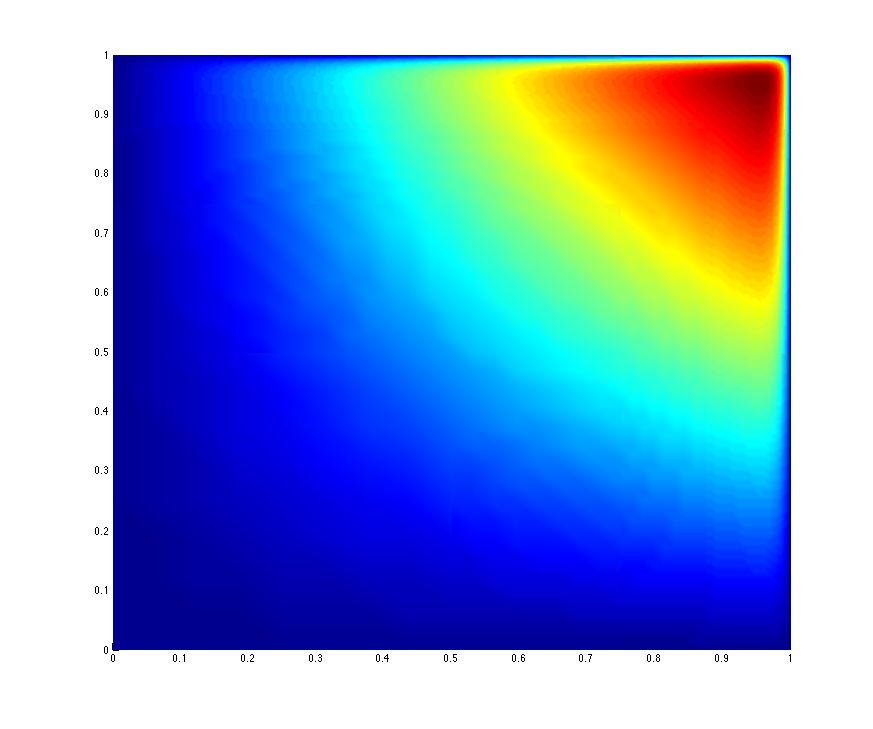
\includegraphics[scale=\oneFig]{figs/Solution12928nomesh.png}
\caption{Computed solution for $\epsilon=10^{-2}$ using a refined mesh.  $L^2$ error is $O(10^{-5})$.}
\end{figure}

We set up our computational experiments by first refining all cells that share an edge with the north and east sides, and repeating this process four times.   We then construct three additional meshes, by uniformly refining every element in the mesh (quadrupling the number of elements each time).  For each of these meshes, we solve on Longhorn, using 1, 4, 16, and 64 nodes, tracking the timing of various portions of the code.  From this data, we extract strong and weak scaling statistics.  

We also used contiguous and discontiguous partitions of each mesh to measure the effect of partition quality on the communication costs in global stiffness matrix assembly.  We created contiguous partitions of the mesh using a HSFC partitioner.  To create the discontiguous partitioning, we chose to use the Zoltan cyclic partitioner, which loops through the list of active elements, sending the first element to the first processor, the next to the next processor, and so on.  After reaching the last processor, the cyclic partitioner cycles back to the first processor and repeats this process.\footnote{Due to the nature of our refinements in this test, a blocked partitioner (equally partitioning the ordered list of active elements by element number) happened to produce nearly-contiguous partitions.  We therefore have omitted this partitioner from our analysis, since we do not believe that its performance here represents its performance in general.}  The cyclic partitioning is a ``worst case" scenario in the sense that each of the current MPI node's elements' neighbors are owned by some other MPI node.

It's worth noting that the runtimes reported here do not represent Camellia running at peak efficiency.  A single Lonestar node contains 12 cores.  Because MPI communication has much higher bandwidth intra-node than inter-node, and for analysis we wanted approximately equal bandwidth between MPI processes, we use only one core per node.  Utilizing all 12 cores on a node would decrease communication costs.  Additionally, there is a parameter within Camellia that controls the batch size for the Trilinos Intrepid batching routines.  Tuning this parameter based on machine-specific cache sizes should further improve performance.

\begin{figure}[h!]
\centering
\subfigure[HSFC partitioning]{
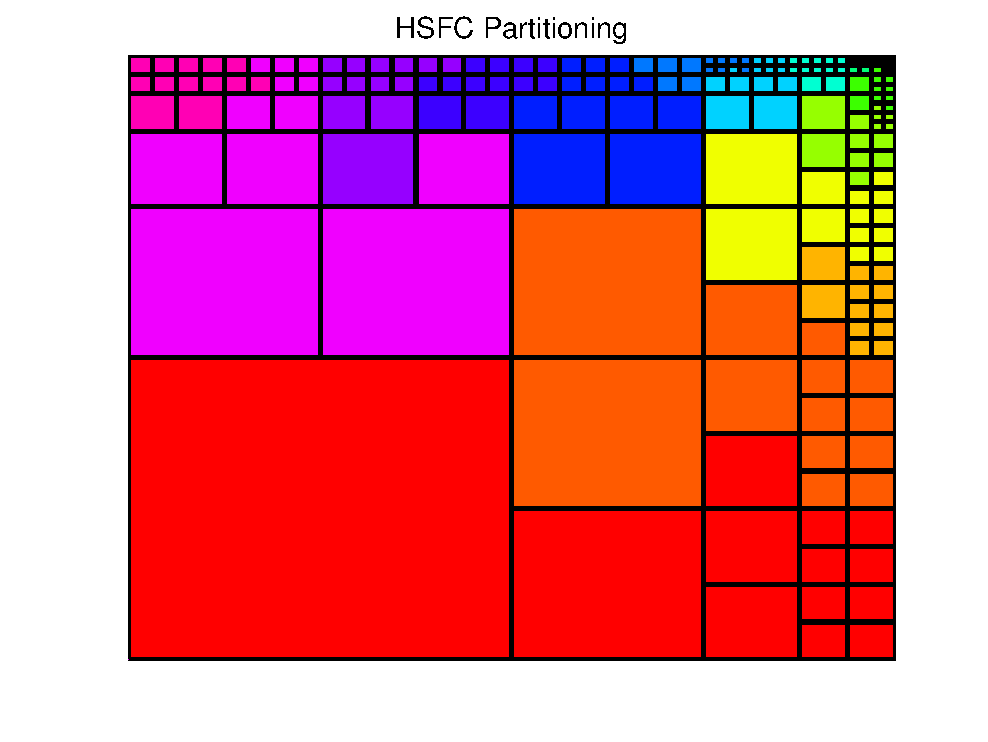
\includegraphics[scale = \twoFig]{figs/hsfc.pdf}
}
\subfigure[Cyclic partitioning]{
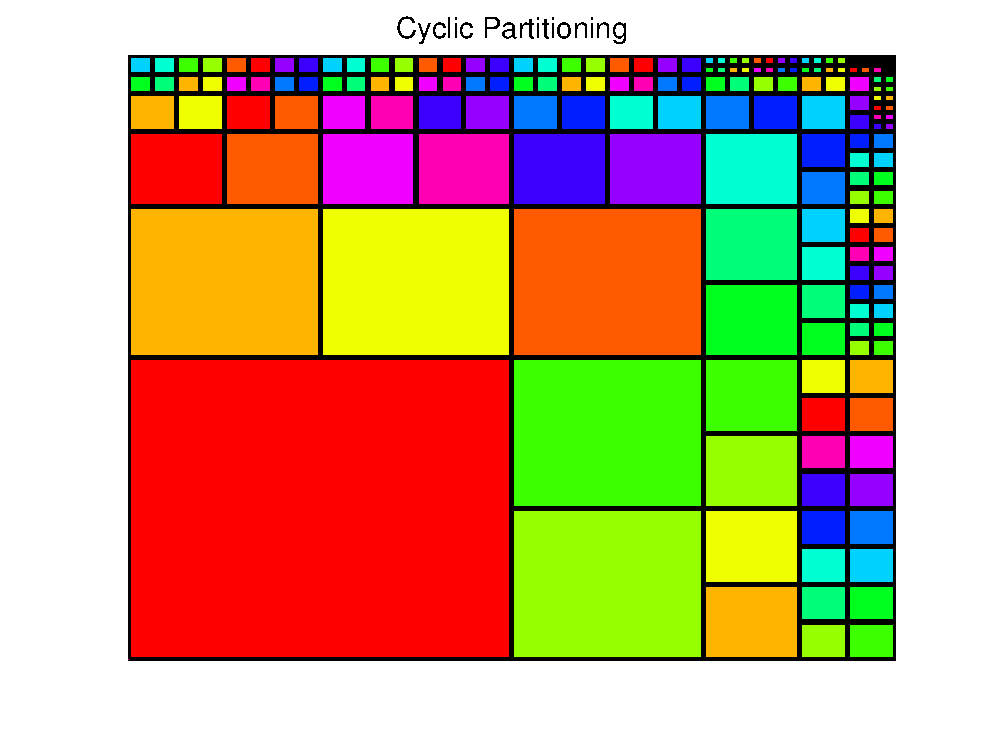
\includegraphics[scale = \twoFig]{figs/cyclic.pdf}
}
\caption{Contiguous and discontiguous partitions of the mesh.}
\end{figure}

\subsection{Weak scaling}

\begin{figure}[h!]
\centering
\subfigure[Local stiffness computation]{
\label{fig:weakScalingStiffness}
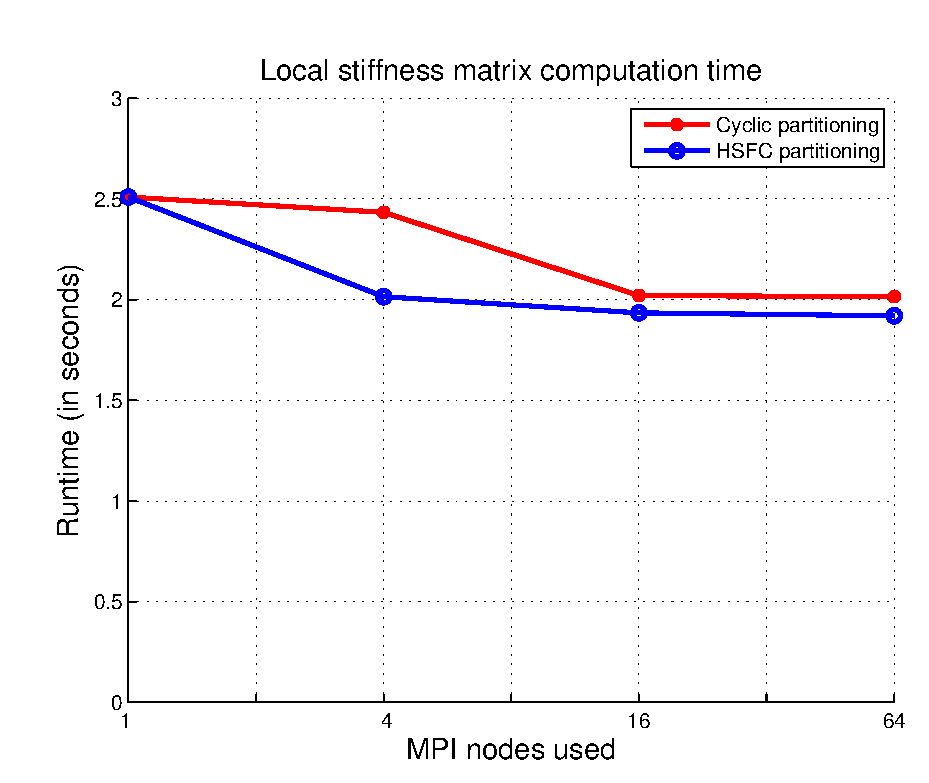
\includegraphics[scale = \twoFig]{figs/scalingFigs/weakScalingLocal.pdf}
}
\subfigure[Global stiffness assembly]{
\label{fig:weakScalingAssembly}
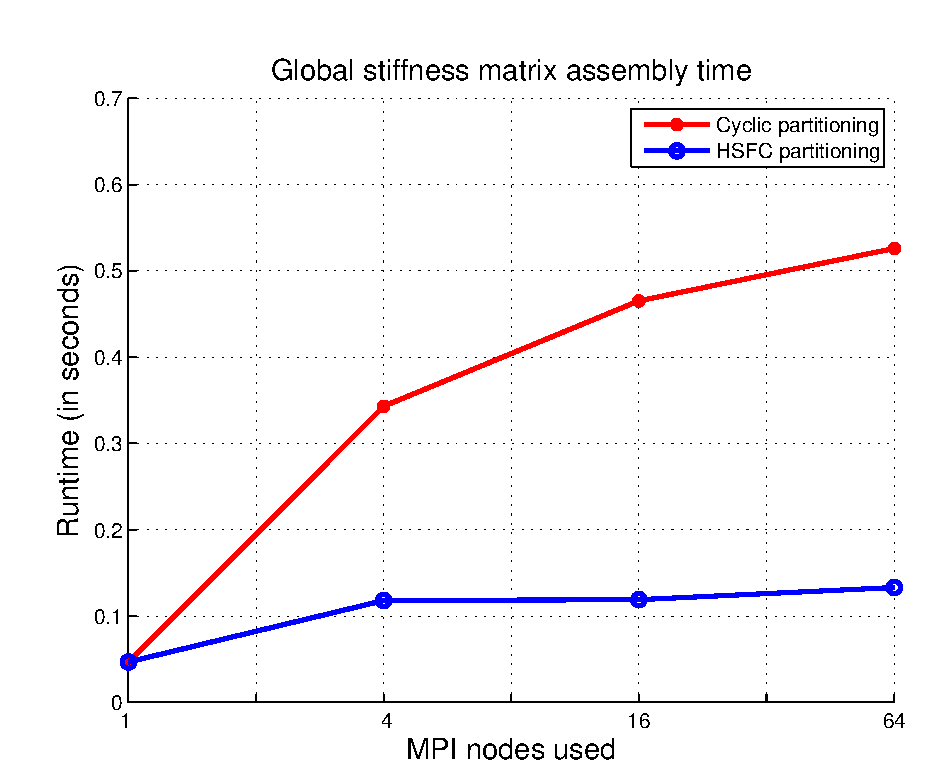
\includegraphics[scale = \twoFig]{figs/scalingFigs/weakScalingAssembly.pdf}
}
\caption{Weak scaling results for computation of local stiffness matrices and global stiffness matrix assembly.  For each run, both the number of MPI nodes and number of elements are increased by a factor of four.}
\end{figure}

The local stiffness computation for both partition types maintain a constant runtime as the problem size and number of processors increase---that is, both achieve weak scalability for this part of the computation, as can be seen in Figure \ref{fig:weakScalingStiffness}.  Assembly of the global stiffness matrix achieves weak scalability only for the contiguous case, as can be seen in Figure \ref{fig:weakScalingAssembly}. It's worth noting, however, that though communication costs grow much faster with a poor partitioning of the mesh, the maximum amount of time spent on assembly is still only a fraction of the time spent on computation of local stiffness matrices.  

\subsection{Strong scaling}
\begin{figure}[h!]
\centering
\subfigure[Global stiffness assembly]{
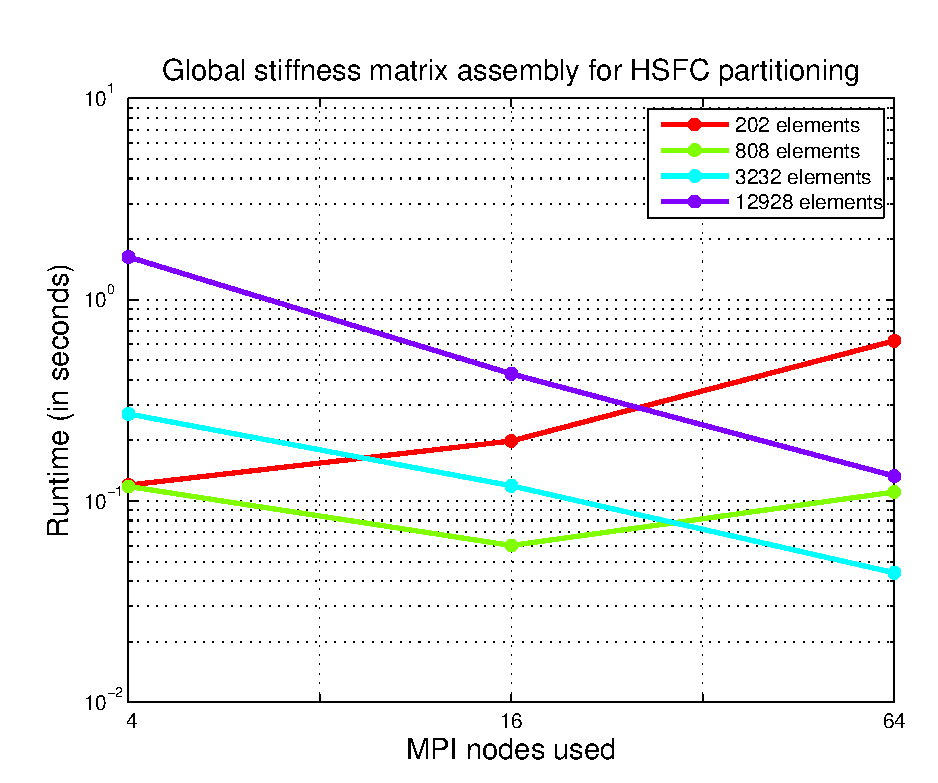
\includegraphics[scale = \twoFig]{figs/scalingFigs/hsfcStrongScalingAssembly.pdf}
}
\subfigure[Local stiffness computation]{
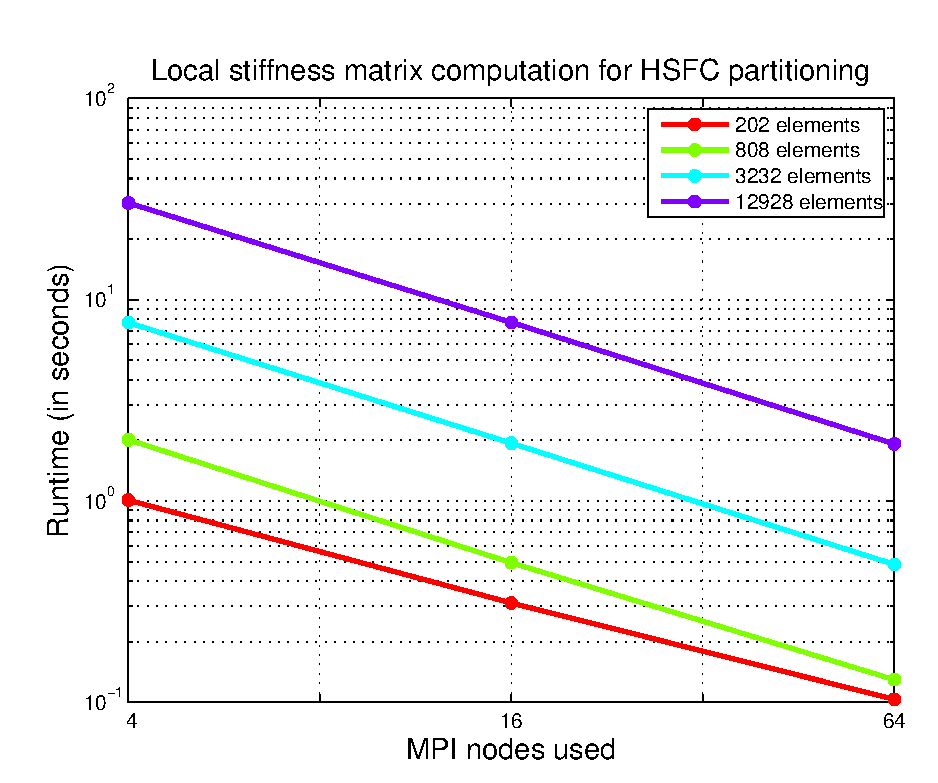
\includegraphics[scale = \twoFig]{figs/scalingFigs/hsfcStrongScalingLocal.pdf}
}
\caption{Strong scaling statistics for a HSFC (localized) partitioning of the mesh.}
\end{figure}

\begin{figure}[h!]
\centering
\subfigure[Global stiffness assembly]{
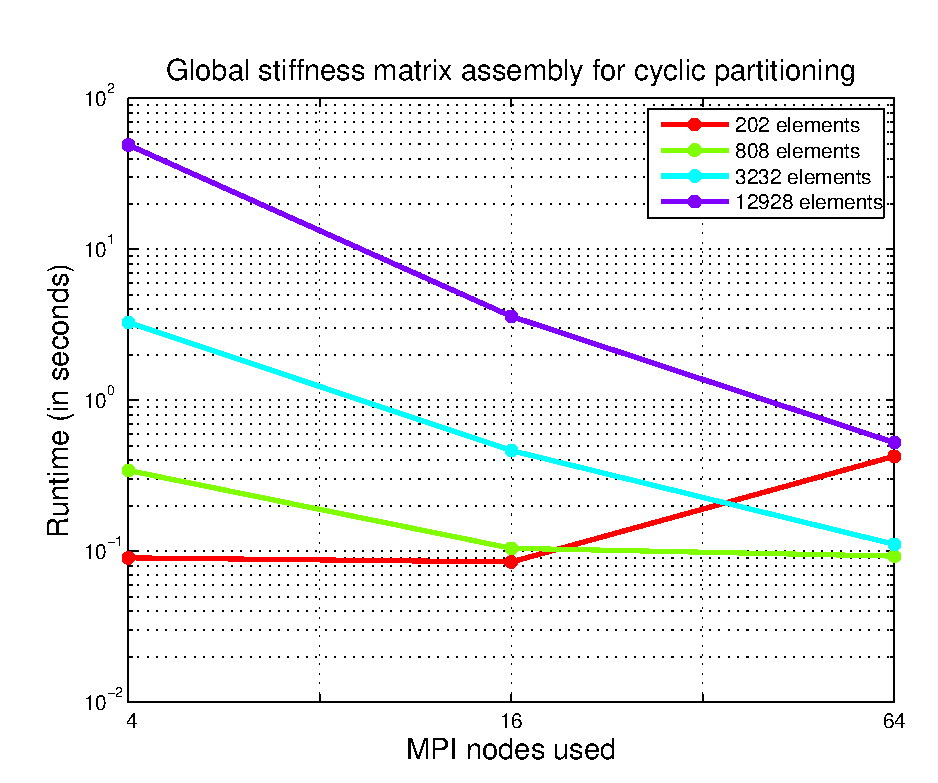
\includegraphics[scale = \twoFig]{figs/scalingFigs/cyclicStrongScalingAssembly.pdf}
}
\subfigure[Local stiffness computation]{
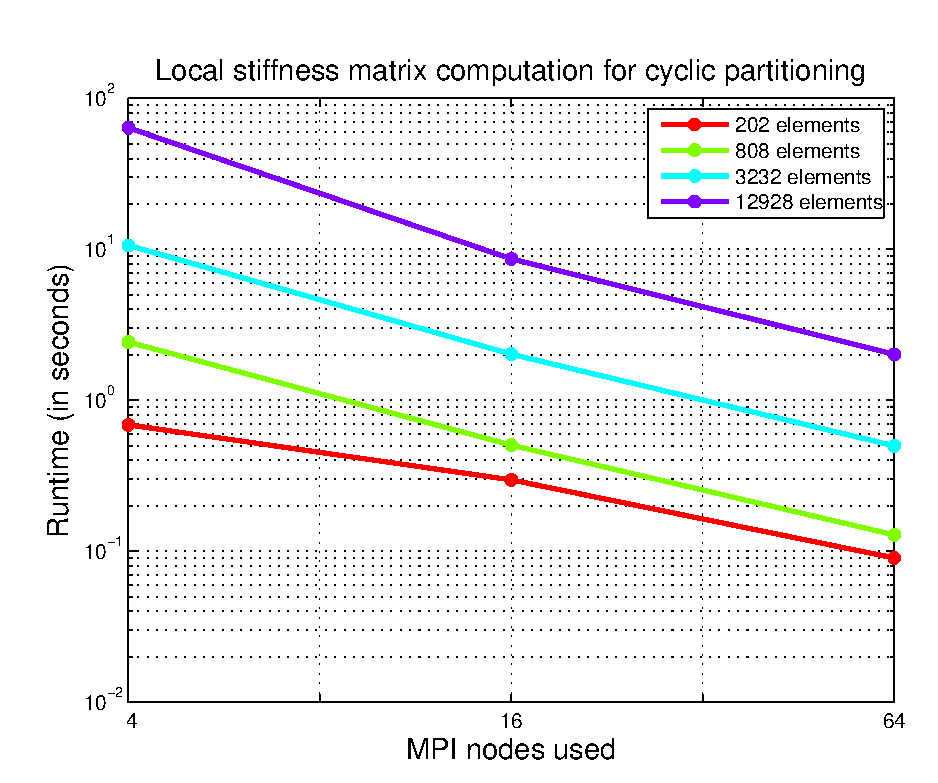
\includegraphics[scale = \twoFig]{figs/scalingFigs/cyclicStrongScalingLocal.pdf}
}
\caption{Strong scaling statistics for a cyclic (non-localized) partitioning of the mesh.}
\end{figure}

\subsection{Breakdown of time spent}

\begin{figure}[h!]
\centering
\subfigure[202 elements, 13343 dofs]{
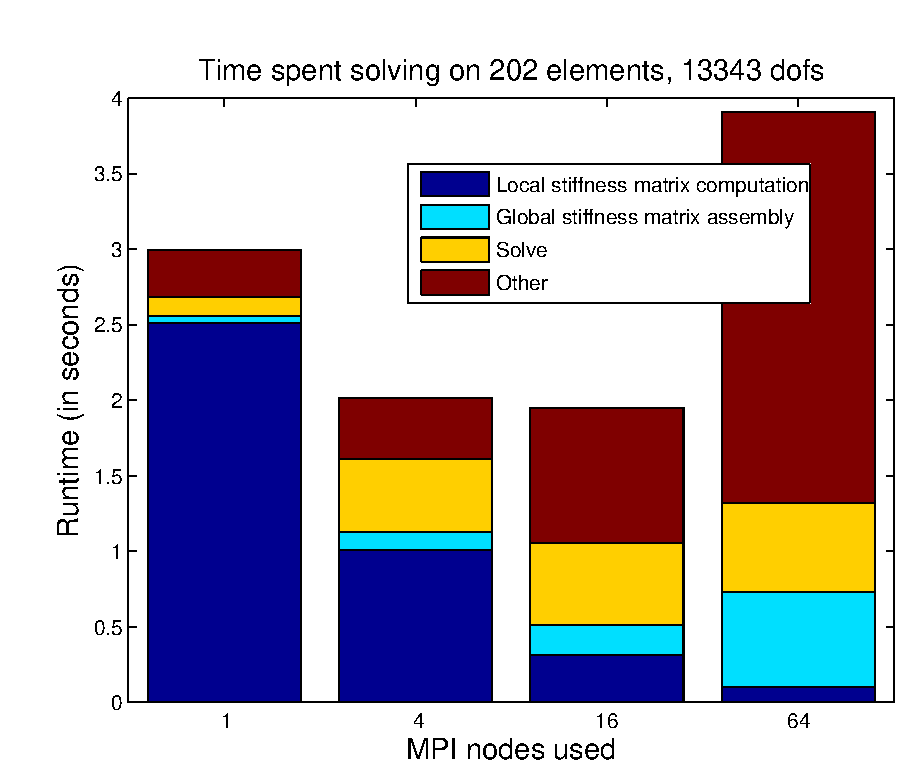
\includegraphics[scale = \fourFig]{figs/scalingFigs/bar_ref0.pdf}
}
\subfigure[808 elements, 52137 dofs ]{
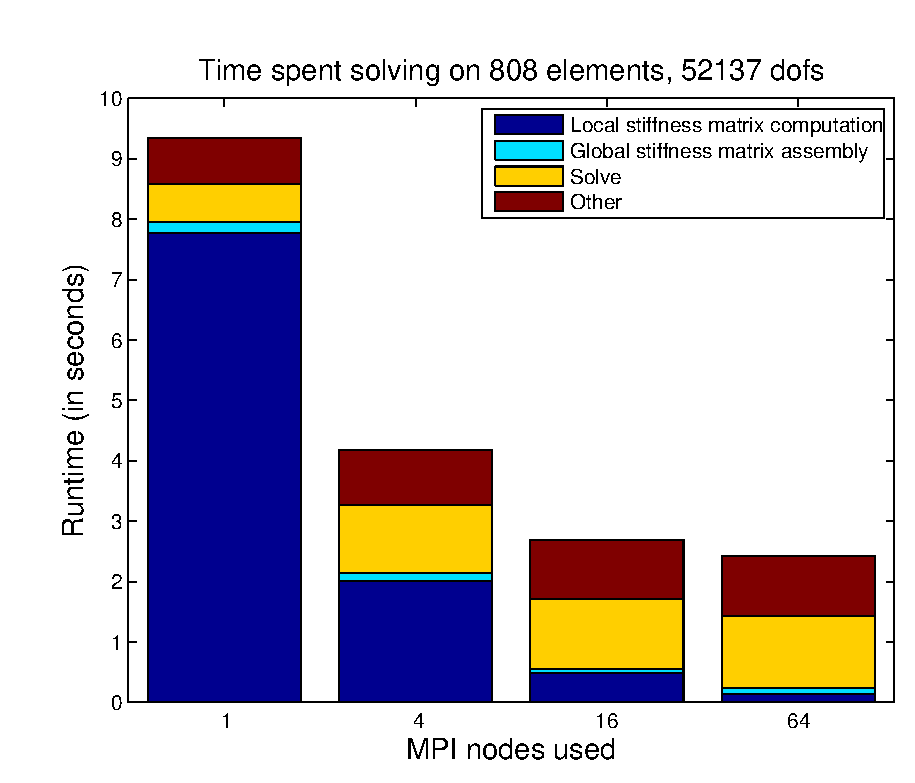
\includegraphics[scale = \fourFig]{figs/scalingFigs/bar_ref1.pdf}
}
\subfigure[3232 elements, 206081 dofs]{
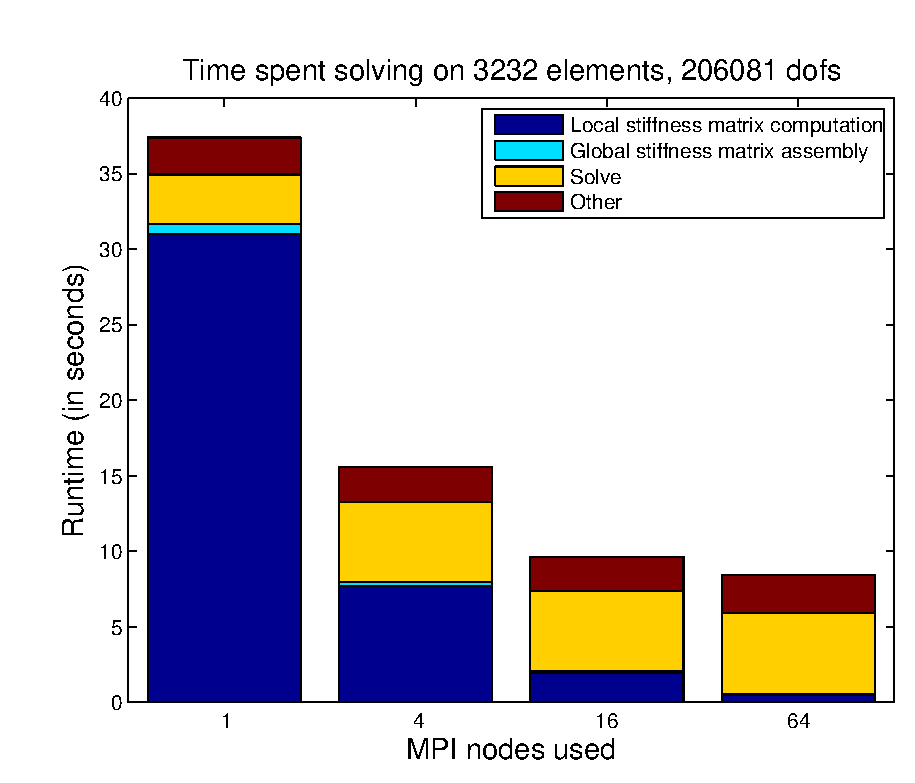
\includegraphics[scale = \fourFig]{figs/scalingFigs/bar_ref2.pdf}
}
\subfigure[12928 elements, 819393 dofs]{
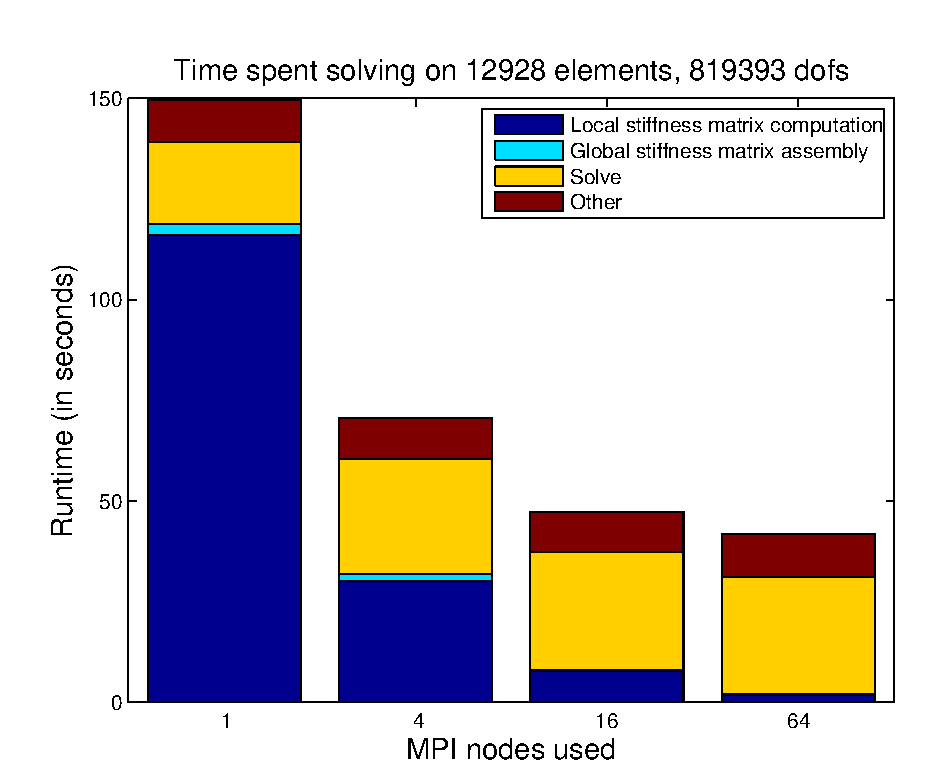
\includegraphics[scale = \fourFig]{figs/scalingFigs/bar_ref3.pdf}
}
\caption{Breakdown of time spent in a solve for a series of HSFC-partitioned meshes.}
\end{figure}

\section{Future work}\label{sec:FutureWork}

\subsection{$hp$-meshes}

The Zoltan partitioner supports a weighted partitioning of a set of objects.  At the moment, every element is treated with equal weight, under the assumption that each contributes an equal number of degrees of freedom.  We would like to extend the partitioning to $hp$-adaptive meshes (where the polynomial order $p$ is allowed to vary element by element) by weighting each element by the number of internal degrees of freedom that it holds.  

\subsection{Parallel solvers}
\subsubsection{MUMPS}

\subsubsection{Conjugate gradients/static condensation}

One benefit of DPG is that the global stiffness matrices it produces are guaranteed to be symmetric positive-definite, allowing for iterative methods like CG to be used. 

Another benefit of the hybridized DG formulation is that the global solve can be reduced down to a solve involving only the flux degrees of freedom. Since the interior degrees of freedom are completely decoupled from each other, the system can be reordered to yield 
\[
\left(\begin{array}{cc}
A &B\\
B^T &C
\end{array}
\right)
\left(\begin{array}{c}
u\\
f
\end{array}
\right) = 
\left(\begin{array}{c}
F\\
G
\end{array}
\right)
\]
where $A$ is block diagonal. Noting that $u = A^{-1}(F-Bf)$, we can substitute this into the second solution to obtain a problem purely in terms of the flux degrees of freedom
\[
(C-B^TA^{-1}B)f = G-B^TA^{-1}F
\]
Since $A$ is easy to invert, and $B$ is a much smaller system, this static condensation would reduce the cost of the solve.

\bibliographystyle{plain}
\bibliography{finalReport}

\end{document}
